\subsection{Kalman CPU}
\label{sec:link2d:kalman-cpu}

The iterative concept for the \locate* approach (described in section~\ref{sec:locate:iterative}) was using the trajectories to predict the future position of each bubble.
As such, it was already performing the \linkDD* task.
For this reason, a modified version was considered as a novel \linkDD* approach.

\subsubsection{Algorithm}

The algorithm starts with an empty list of previously found bubbles.
It then loops over these steps, for each frame in the video:
\begin{enumerate}
	\itemsep 0em
	\item Store the positions of the located bubbles in a suitable data structure. Based on the settings, a basic coordinate list or a 2D binary tree could be used;
	\item For each bubble in the ``previous bubbles'' list:
	      \begin{enumerate}
		      \item Compute its velocity and acceleration from the last trajectory points, if available;
		      \item Compute a predicted position;
		      \item Find the candidate bubbles in the next frame:
		            \begin{itemize}
			            \item If the binary tree was used as representation, consider all bubbles within a \textit{delta} from the predicted position;
			            \item If the bubbles list was used as representation, consider all bubbles;
		            \end{itemize}
		      \item Among the candidates, chose the closest one (in terms of Manhattan distance) to the predicted position;
		      \item Check that the distance of the match is reasonable:
		            \begin{itemize}
			            \item If it is, link the two bubbles, and mark the chosen one as linked;
			            \item If it is not, consider the bubble lost for this frame. If the bubble is lost for multiple consecutive frames, it is removed from the list;
		            \end{itemize}
	      \end{enumerate}
	\item Add all unlinked bubbles to the list, as new tracklets.
\end{enumerate}
The 2D binary tree was added to reduce the amount of possible matches, by splitting the coordinates into 4 bins for every node layer, storing the bins as Python lists.
To obtain the bubbles within a \textit{delta} from the predicted position, the tree would consider all bins that (at least partially) satisfied the condition.

\subsubsection{Evaluation}

Considering the tree choice, it was possible to choose between:
\begin{itemize}
	\itemsep 0em
	\item no tree at all: as stated in the algorithm overview, the original \texttt{NumPy} array of bubbles was used as set of candidates;
	\item tree with 0 layers: no split was performed, therefore the original \texttt{NumPy} array was simply translated into a Python list. The distance computation is the same as with no tree, with added overhead of creating and accessing the Python list instead of the \texttt{NumPy} array.
	\item tree with maximum number of layers: each leaf bin represents a single pixel of the original image, therefore will contain either 1 or 0 bubbles. The number of layers is $\lceil log_2(P) \rceil$, where $P$ is the side, in pixels, of the captured image. In our case, $P{=}960$, prompting to choose 9 layers. This option has the most fine-grained way to choose the bubbles at a specific distance. It however adds the most overhead related both to constructing a bigger tree, and traversing multiple paths to construct the set of bubbles to be evaluated.
	\item tree with intermediate number of layers: this is a compromise between efficiency in building and using the tree, and reducing the number of distances to compute.
\end{itemize}
These different approaches are compared in figure~\ref{fig:linkDD:kalmancpu:speed-cmp}: when considering the tree, the best choice is a compromise between granularity and tree complexity.
However, the overhead of building the tree does still not match the performance without it, thanks to the extreme optimization of the \texttt{NumPy} library.
As such, the version with no tree was the chosen one.

\begin{figure}
	\centerline{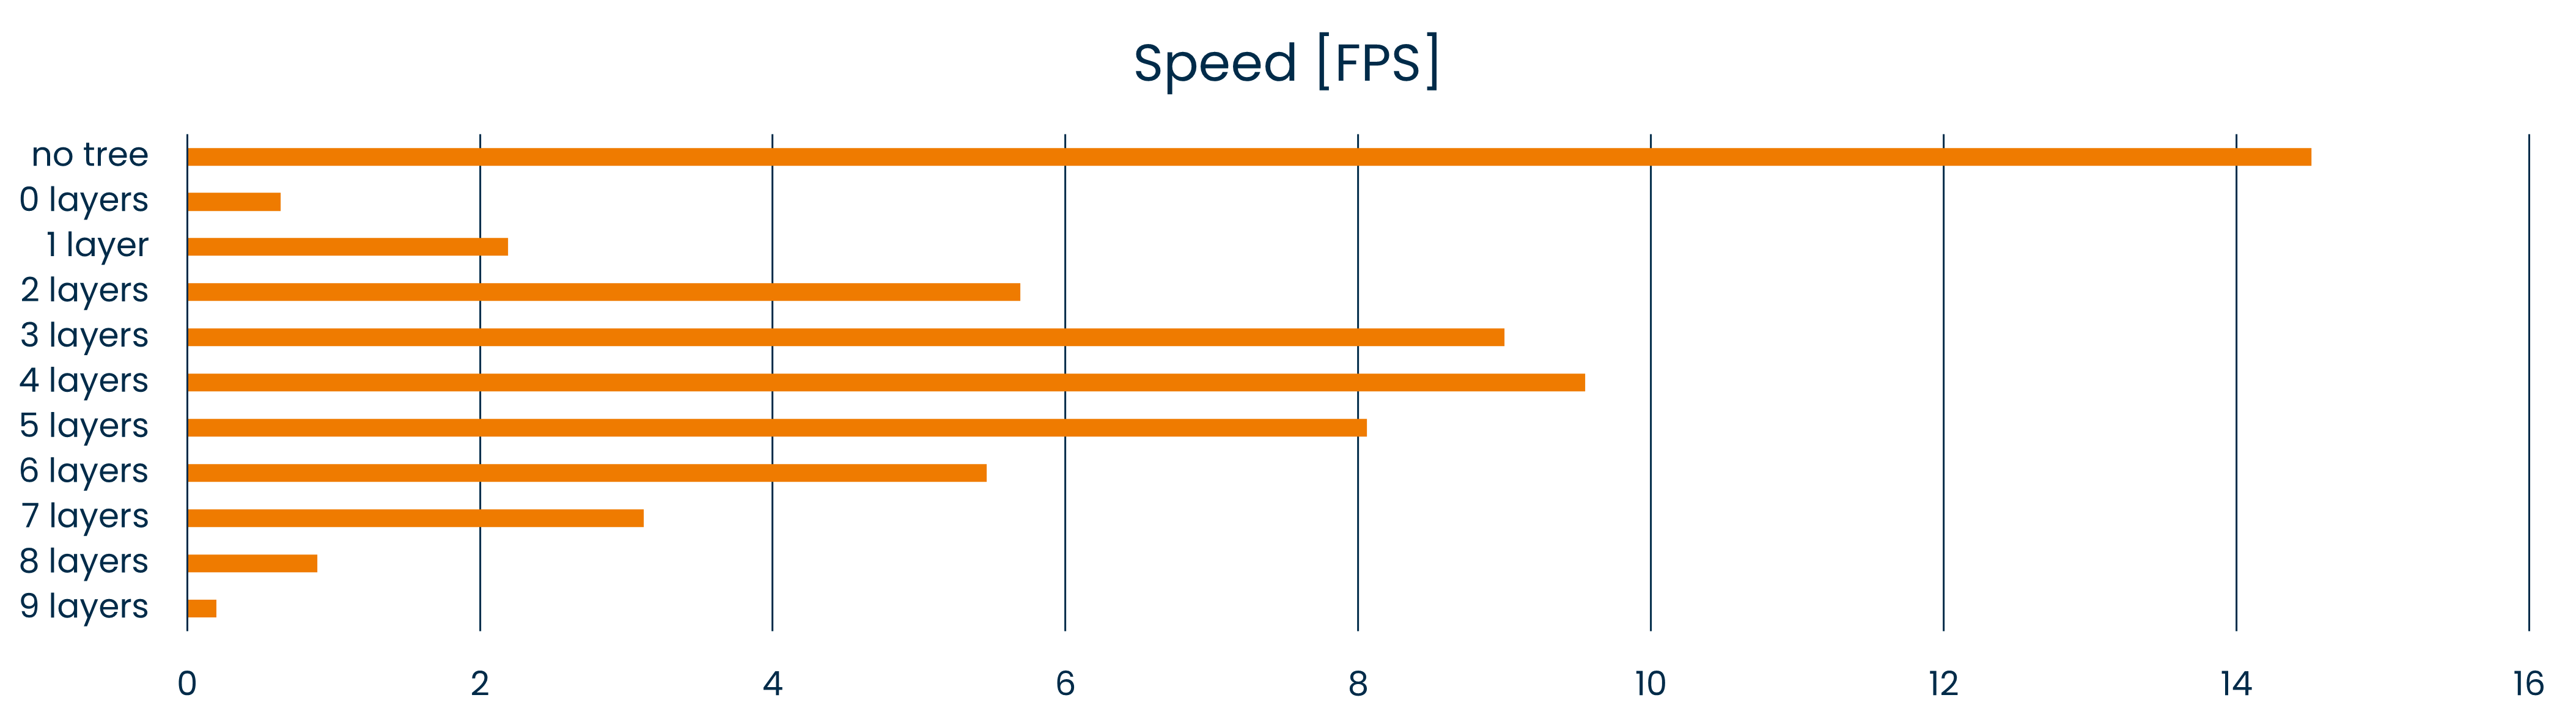
\includegraphics[width=\locateimgsize]{images/link-2dtree-speeds.png}}
	\caption{\centering Comparing speeds for different tree sizes in the Kalman CPU \linkDD* approach}
	\label{fig:linkDD:kalmancpu:speed-cmp}
\end{figure}

As visible in figure~\ref{fig:linkDD:kalmancpu:speed-cmp}, the overall speed is limited to about 14 FPS, much slower than Trackpy.
On top of that, the result is also slightly worse: while it looks good at visual inspection (see figure~\ref{fig:linkDD:kalmancpu}), the total number of traces is higher than Trackpy, at about 8400 tracklets found.

\begin{figure}[H]
	\centerline{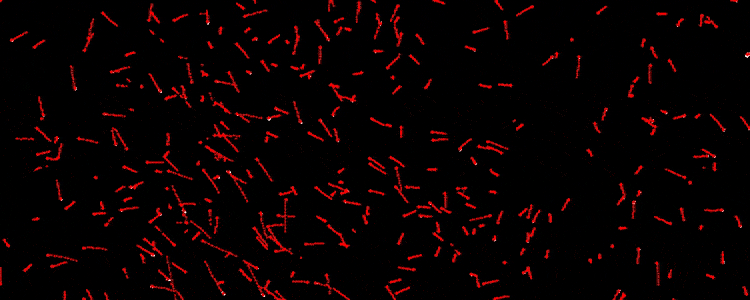
\includegraphics[width=\locateimgsize]{images/link2d/kalman_CPU.png}}
	\caption{\centering A frame from the Kalman CPU \linkDD* result, full video available at~\cite{linkDD-kalman-cpu}}
	\label{fig:linkDD:kalmancpu}
\end{figure}
